%%%%%%%%%%%%%%%%%%%%%%%%%%%%%%%%%%%%%%%%%
% University Assignment Title Page 
% LaTeX Template
% Version 1.0 (27/12/12)
%
% This template has been downloaded from:
% http://www.LaTeXTemplates.com
%
% Original author:
% WikiBooks (http://en.wikibooks.org/wiki/LaTeX/Title_Creation)
%
% License:
% CC BY-NC-SA 3.0 (http://creativecommons.org/licenses/by-nc-sa/3.0/)
% 
% Instructions for using this template:
% This title page is capable of being compiled as is. This is not useful for 
% including it in another document. To do this, you have two options: 
%
% 1) Copy/paste everything between \begin{document} and \end{document} 
% starting at \begin{titlepage} and paste this into another LaTeX file where you 
% want your title page.
% OR
% 2) Remove everything outside the \begin{titlepage} and \end{titlepage} and 
% move this file to the same directory as the LaTeX file you wish to add it to. 
% Then add \input{./title_page_1.tex} to your LaTeX file where you want your
% title page.
%
%%%%%%%%%%%%%%%%%%%%%%%%%%%%%%%%%%%%%%%%%
%\title{Title page with logo}
%----------------------------------------------------------------------------------------
%	PACKAGES AND OTHER DOCUMENT CONFIGURATIONS
%----------------------------------------------------------------------------------------

\documentclass[12pt]{article}
\usepackage[english]{babel}
\usepackage[utf8x]{inputenc}
\usepackage{amsmath}
\usepackage{graphicx}
\usepackage[colorinlistoftodos]{todonotes}
\usepackage{upgreek}

\begin{document}

\begin{titlepage}

\newcommand{\HRule}{\rule{\linewidth}{0.5mm}} % Defines a new command for the horizontal lines, change thickness here

\center % Center everything on the page
 
%----------------------------------------------------------------------------------------
%	HEADING SECTIONS
%----------------------------------------------------------------------------------------

\textsc{\LARGE NITK SURATHKAL}\\[1.5cm] % Name of your university/college
\textsc{\Large Digital Signal Processing}\\[0.5cm] % Major heading such as course name
\textsc{\large Mini Project}\\[0.5cm] % Minor heading such as course title

%----------------------------------------------------------------------------------------
%	TITLE SECTION
%----------------------------------------------------------------------------------------

\HRule \\[0.4cm]
{ \huge \bfseries Adaptive Beamforming}\\[0.4cm] % Title of your document
\HRule \\[0.5cm]
 
%----------------------------------------------------------------------------------------
%	AUTHOR SECTION
%----------------------------------------------------------------------------------------

\begin{minipage}{0.4\textwidth}
\begin{flushleft} \large
\emph{Authors:}\\
Aniket \textsc{Rege}\\
Prabhanjan \textsc{Mannari}\\
Ritesh \textsc{Waykole}\\% Your name
\end{flushleft}
\end{minipage}
~
\begin{minipage}{0.4\textwidth}
\begin{flushright} \large
\emph{Supervisor:} \\
Dr. Pathipati \textsc{Srihari} % Supervisor's Name
\end{flushright}
\end{minipage}\\[1cm]

% If you don't want a supervisor, uncomment the two lines below and remove the section above
%\Large \emph{Author:}\\
%John \textsc{Smith}\\[3cm] % Your name

%----------------------------------------------------------------------------------------
%	DATE SECTION
%----------------------------------------------------------------------------------------

{\large \today}\\[1cm] % Date, change the \today to a set date if you want to be precise

%----------------------------------------------------------------------------------------
%	LOGO SECTION
%----------------------------------------------------------------------------------------

\includegraphics{NITK-Emblem.jpg}\\[1cm] % Include a department/university logo - this will require the graphicx package
 
%----------------------------------------------------------------------------------------

\vfill % Fill the rest of the page with whitespace

\end{titlepage}


\begin{abstract}
Adaptive array antennas use smart signal processing algorithms to allow the antenna to steer the beam to any direction of interest while simultaneously nulling interfering signals. Beamforming is the technique used to create the radiation pattern of the array by constructively adding the phases of the signals in the direction of targets and nulling the pattern of undesired/interfering targets, thus providing directional sensitivity without physically moving an array of receivers and transmitters. This can be implemented with a simple FIR tapped delay line filter, whose weights may be changed adaptively to provide optimal beamforming, which reduced the Minimum Mean Square Error (MMSE) between the actual and desired beam pattern. The most common Adaptive beamforming algorithms explored are LMS algorithm and RLS algorithm, of which the LMS algorithm is explored in this project. The LMS algorithm is described by a recursive equation which updates filter weights in such a manner that they converge to the optimum filter weight in an inverse accordance with the gradient of the mean square error vs. filter weight curve, i.e. changing the weights in a direction opposite to that of gradient slope. We hope to explore these techniques and create our own modification to existing algorithms for a more efficient beamforming process. 
\end{abstract}

\section{\LARGE Preliminaries}

The following results are given as preliminaries for the purpose of foresight into the theoretical principles behind adaptive beamforming and its use in antenna arrays.

\subsection{Random Process}

A random process X(t,s) is an ensemble of time functions from the sample space S. \\The samples $X_{ti} = x(ti), i = 1, 2, 3, \cdots n$ are n random variables characterized by their joint probability density function = $p(x_{t1}, x_{t2}, \cdots x_{tn})$

\subsection{Stationary Random Process}

Consider random process $X(ti) = x(ti), i = 1, 2, 3, \cdots n$ and \\
$X(ti + \uptau) = X(ti + \uptau, i = 1, 2, 3, \cdots n$ for some parameter $\uptau$ with probability density functions \\ 
\indent $p(x_{t1}, x_{t2}, x_{t3}, \cdots x_tn) = p_1$ \\
\indent $p(x_{t1+\uptau}, x_{t2+\uptau}, x_{t3+\uptau}, \cdots x_{tn+\uptau}) = p_2$ \\
We say the process x(ti) is stationary  if $p_1 = p_2 \forall n $

%\todo[inline, color=green!40]{This is an inline comment.}

\subsection{Statistical [Ensemble] Averages}
Consider a random process $X(t_i) = x(t_i)$ sampled at $t = t_i$\\ $X(t_i)$ is a random variable.
The $l^{th}$ moment of the random variable is defined as the expected value of $x^l(t_i)$ \\
\indent $$E[X^l(t_i)] = \int_{-\infty}^{\infty} X_{ti}^l p(x_{ti}) dx_{ti}$$
If the process is stationary, $p(x_{ti}) = p(x_{ti + \uptau})$ and hence the $l^{th}$ moment is a constant. The statistical mean or expected value of a random process is defined as $$\mu_{x}(t_i) = \int_{-\infty}^{\infty} x_{ti} p(x_{ti}) dx_{ti}$$

\subsection{Correlation}
The statistical correlation between two random variables of the process is defined as $$ E(X_{t1}X_{t2}) = \int_{-\infty}^{\infty} \int_{-\infty}^{\infty} x_{t1}x_{t2} p(x_{t1}x_{t2})dx_{t1}dx_{t2}$$

if $t_2 = t_1 + \uptau$, the above relation is known as the auto-correlation of the random process $x(t_i)$ denoted as $r_{xx}(t_1,t_{1+\uptau})$
$$r_{xx}(t_1,t_{1+\uptau}) = \int_{-\infty}^{\infty} \int_{-\infty}^{\infty} x_{t1}x_{t1 + \uptau} p(x_{t1}x_{t1 + \uptau})dx_{t1}dx_{t1 + \uptau}$$
Suppose the mean $\mu_x(t_i)$ is constant, i.e. independent of $t_i$ and the auto-correlation depends only on the lag $\uptau$ and is independent of $t_i$, then the random process $X(t_i)$ is said to be stationary in the wide sense, or \textbf {Wide Sense Stationary}.

\subsection{Auto Covariance of a Random Process}

$$ C_{xx}(t_1,t_2) = E([X_{t1}-\mu_{t1}][X_{t2}-\mu_{t2}])\\ =r_{xx}(t_1,t_2) - \mu_{t1}\mu_{t2} $$    

For a stationary random process, $e_{xx}(\uptau) = r_{xx}(\uptau) - \mu^2 $

\subsection{Statistical Averages for Joint Random Processes}
Let X(t) and Y(t) be two random processes characterized by joint PDF $P(x_{t1}, x_{t2}, \cdots y_{t1},y_{t2}, \cdots ) $ We define \\ \textbf{Cross Correlation: } $$ r_{xy}(t_1,t_2) = \int_{-\infty}^{\infty} \int_{-\infty}^{\infty} x_{t1}y_{t2} p(x_{t1}y_{t2})dx_{t1}dy_{t2}$$
\textbf{Cross Covariance: } $$ r_{xy}(t_1,t_2) = \mu_y(t_2)\mu_x(t_1)$$

%\begin{table}
%\centering
%\begin{tabular}{l|r}
%Item & Quantity \\\hline
%Widgets & 42 \\
%Gadgets & 13
%\end{tabular}
%\caption{\label{tab:widgets}An example table.}
%\end{table}

\subsection{Power Density Spectrum}

A stationary random process is an infinite energy signal, and hence does not have a Fourier transform. Its spectral characteristic is obtained from the Fourier Transform of it auto-correlation according to Wiener-Khinchin theorem.
\\ \textbf{State Theorem: }
\begin{align*}
 \Gamma_{xx}(F) &= \int_{-\infty}^{\infty} r_{xx}(\tau)e^{-j2\pi F\tau} d\tau\\
 r_{xx}(\tau) &= \int_{-\infty}^{\infty} \Gamma_{xx}(F)e^{-j2\pi F\tau} dF \\
 				&= \int_{-\infty}^{\infty} \Gamma_{xx}(F) dF \\
				&= E(x^2_t)  \geq 0 \\
 \end{align*}
$r_{xx}$(0) is equal to average power of the random process

\subsection{Discrete Time Random Signals}
We model a discrete time random signal using a discrete time random process which is atleast wide sense stationary (possible with zero mean).
Consider a random signal x[n] of length N, we define its auto-correlation as
\begin{align*}
 r_{xx}(l) &= \sum_{n=0}^{N} x[n]x[n-l] \\
 r_{xx}(m) &= E(x[n]x*[n-m]) 
\end{align*}
\subsection{Vector Space Treatment of Random Variables}
Consider a vector of random variables x, with mean $\mu_x$
\[
\mathbf{x}=
  \begin{bmatrix}
    x_1 \\
    x_2 \\
    x_3 \\
    \vdots \\
    x_n
  \end{bmatrix}
  \indent\indent \mathbf{\mu_x} =
  \begin{bmatrix}
    \mu_{x1} \\
    \mu_{x2} \\
    \mu_{x3} \\
    \vdots \\
    \mu_{xn}
  \end{bmatrix}
\]
We define the auto-covariance matrix $C_{p\times p}$ as $$ C_{p\times p} = E[(\mathbf{x}-\mathbf{\mu_x})(\mathbf{x}-\mathbf{\mu_x})^H]$$
where $a^H$ is the \textbf{Hermitian} of a. Consider a random process x

Consider a random process \[
\mathbf{x}=
  \begin{bmatrix}
    x[n] \\
    x[n-1] \\
    x[n-2] \\
    \vdots \\
    x[n-p]
  \end{bmatrix}
\]

We define the auto-correlation matrix $R_{xx}$ as $$ R_{xx} = E[\mathbf{x}\mathbf{x^H}]$$ 
We note that $C_p\times p$, $R_{xx}$, i.e. the auto-covariance and the auto-correlation matrices are Hermitian. Further, $R_{xx}$, the auto-correlation matrix, is \textbf{Hermitian Toeplitz} if $\mathbf{x}$ is wide sense stationary.

\subsection{Properties of Hermitian Matrices}


The Eigenvalues $\lambda_i$ are real and the eigenvectors are orthogonal.

Let $\mathbf{T}_{P\times P}$ be a Hermitian Matrix and let $\mathbf x$ be the eigenvector for eigenvalue $\lambda$.
\indent Then $\mathbf{T}\mathbf{x} = \lambda \mathbf{x}$

Take Hermitian on both sides and multiply by $\mathbf{x}$
$$\mathbf{x}^H \mathbf{T}^H \mathbf{x} = \lambda^*\mathbf{x}^H\mathbf{x}$$
But $\mathbf{T}^H=\mathbf{T}$ and $\mathbf{T}\mathbf{x} = \lambda \mathbf{x}$
$$\mathbf{x}^H\lambda\mathbf{x} = \lambda^*\mathbf{x}^H\mathbf{x}$$
\indent $\Longrightarrow \lambda = \lambda^k$ \indent Hence eigenvalues are real.\\
Consider 
\begin{align*}
T\mathbf{x_1} &= \lambda_1\mathbf{x_1}\cdots\cdots\cdots(1) \indent (\lambda_1 \neq \lambda_2) \\
T\mathbf{x_2} &= \lambda_1\mathbf{x_2}\cdots\cdots\cdots(2)
\end{align*}
Take Hermitian of (1) and multiply by $\mathbf{x_2}$
\begin{align*}
\mathbf{x_1}^HT\mathbf{x_2} &= \lambda_1\mathbf{x_1}^H\mathbf{x_2}\\
\mathbf{x_1}^H\lambda_2\mathbf{x_2} &= \lambda_1\mathbf{x_1}^H\mathbf{x_2}\\
(\lambda_2 - \lambda_1)&\mathbf{x_1}^H\mathbf{x_2} = 0
\end{align*}

But $(\lambda_2 \neq \lambda_1) \Rightarrow \mathbf{x_1}^H\mathbf{x_2}=0$ \\
Hence the eigenvectors are orthogonal.

Say $\lambda_1\neq\lambda_2\neq\lambda_3\neq\cdots\neq\lambda_p$ with eigenvectors $\mathbf{e_1},\mathbf{e_2},\cdots,\mathbf{e_p}$
Eigenvalues of $\mathbf{T}$ are:
\begin{align*}
[\mathbf{e_1},\mathbf{e_2},\cdots,\mathbf{e_p}] &= [\lambda_1\mathbf{e_1},\lambda_2\mathbf{e_2},\cdots,\lambda_p\mathbf{e_p}] \\
\mathbf{T}\mathbf{E}&=\mathbf{E}\mathbf{D}
\end{align*}
where $\mathbf{E}$ is the matrix with eigenvectors as columns and $\mathbf{D}$ is the diagonal matrix of eigenvalues.
Suppose the eigenvectors are normalized,\\\\
\indent$\mathbf{E}^H\mathbf{E} =\mathbf{T}$ [$\mathbf{E}$ is unitary]\\
then $\mathbf{T}\mathbf{E} = \mathbf{E}\mathbf{D}$\\ multiply by $\mathbf{E}^H$ \\
\begin{align*}
\mathbf{T}\mathbf{E}\mathbf{E}^H &= \mathbf{E}\mathbf{D}\mathbf{E}^H \\
\mathbf{T}&=\mathbf{E}\mathbf{D}\mathbf{E}^H
\end{align*}
-\textbf{Similarity Transform}
\\\\Note that det(t) = det(n)
\\\\A matrix $\mathbf{A}_{n\times n}$ is said to be \textbf{positive semi definite} if for any non zero vector, $x\neq\theta_n$
$$\mathbf{x}^HA\mathbf{x}\geq 0$$
We note that covariance and correlation matrices are at least PSD.

\subsection{Orthogonality Principle}
Orthogonality Principle states that the error e[n] between the desired signal d[n] and the estimator signal is minimum in the least square sense if the error e[n] is orthogonal to x[n], i.e. $$E[\mathbf{x}[n]\mathbf{e}[n]]=0$$
Even using this condition, we arrive at the same equation for optimum filter weights
$$h_opt = R^{-1}P$$
R- auto-correlation matrix\\
P- cross correlation matrix

\section{Adaptive Filters}

Filters with adjustable coefficients, called adaptive filters, are employed. Such filters incorporate algorithms that allow the filter coefficients to adapt to the signal statistics. Adaptive filters self learn. As the signal into the filter continues, the adaptive filter coefficients adjust themselves to achieve the desired result, such as identifying an unknown filter or canceling noise in the input signal. Filter parameters are shown in Figure 1. We choose an input signal x(n) and a desired level d(n), such that our filter (with transfer function h(n) ) output y(n) is the best possible estimate of d(n). Reducing the error in estimation is a key component of our adaptive filtering process.
Some practical applications of adaptive filters are listed below.
% Commands to include a figure:
\begin{figure}[!ht]
\centering
\includegraphics[width=0.5\textwidth]{adaptive_filter.png}
\caption{\label{fig:adaptive_filter}Block diagram for an adaptive filter.}
\end{figure}

\subsection{Adaptive Line Enhancer}
This example shows how to apply adaptive filters to signal separation using a structure called an adaptive line enhancer (ALE). In adaptive line enhancement, a measured signal x(n) contains two signals, an unknown signal of interest v(n), and a nearly-periodic noise signal $\eta(n)$.The goal is to remove the noise signal from the measured signal to obtain the signal of interest. 

Say our signal of interest $$v(n)= Acos(\omega_cn)$$ and our noise signal is $$\eta(n)$$In the simplest case, we would implement a bandpass filter centered at the frequency of oscillation of our signal of interest $\omega_c$ (shown in Figure 2) to extract the signal $v(n)$

\begin{figure}[!ht]
\centering
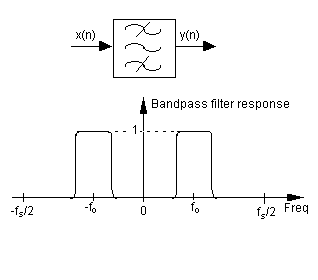
\includegraphics[width=0.5\textwidth]{bandpass_filter.png}
\caption{\label{fig:bandpass_filter}Spectrum for a bandpass filter centered at frequency $f_c$.}
\end{figure}

Now suppose the frequency of oscillation $\omega_c$ is time variant. In this case our filter will be of no use. Thus we need a filter to be \textbf{adaptive}, or robust to such unpredictable changes.The Discrete Time Fourier Transform of our signal of interest $v(n)$ is given in Figure 3. It is called the \textbf{line spectra} of the discrete time function $v(n)$, as it consists of lines centered at frequencies f and -f. Our narrowband filter will allow and enhance these lines centered at frequency $w_c$ or f, and filter out the noise. Since the filter is enhancing the lines of the line spectra, this type of filter is known as an \textbf{Adaptive Line Enhancer}.

\begin{figure}[!ht]
\centering
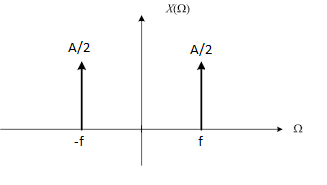
\includegraphics[width=0.5\textwidth]{cosinedtft.png}
\caption{\label{fig:cosinedtft}Line spectrum our signal of interest $v(n)$, centered at $w_c$/f}
\end{figure}


An adaptive line enhancer (ALE) is based on the straightforward concept of linear prediction. A nearly-periodic signal can be perfectly predicted using linear combinations of its past samples, whereas a non-periodic signal cannot. Now in terms of adaptive filter parameters x(n) and d(n), a delayed version of the measured signal $s(n-D)$ is used as the reference input signal x(n) to the adaptive filter, and the desired response signal d(n) is made equal to s(n). The parameters to choose in such a system are the signal delay D and the filter length L used in the adaptive linear estimate. The amount of delay depends on the amount of correlation in the signal of interest. Since we don't have this signal(this is what we are estimating in this application), a value of D is chosen arbitrarily and varied later.
\section{Beamforming}
Consider a two-element antenna array. The
array consists of two omnidirectional (equally sensitive to all directions) antennas A and
B, as shown in Figure 4. A desired signal $s(n) = \alpha(n) cos(n\omega_o + \phi_1)$ arrives in the
direction perpendicular to the line connecting A and B. An interferer (jammer) signal
$v(n) = \beta(n) cos(n\omega_o+ \phi_2)$ arrives at an angle $\theta_o$ relative to s(n). The signal sequences
s(n) and v(n) are assumed to be narrow-band processes with random phases $\phi_1$ and $\phi_2$,
respectively. It is also assumed that the random amplitudes $\alpha$(n) and $\beta$(n) are zero-mean
and uncorrelated with each other. The two omnis are separated by a distance of l = $\lambda_c$/2
meters, where $\lambda_c$ is the wavelength associated with the continuous time carrier frequency
$$\omega_c = \dfrac{\omega_o}{T}$$


with T being the sampling period. The coefficients, h0 and h1, of the beamformer are
adjusted, so that the output error, e(n), is minimized in the mean-square sense.
The adaptive beamformer of below figure is characterized by the
following signal sequences:
\begin{enumerate}
\item Primary input
$$d(n) = \alpha(n) cos(n\omega_o + \phi_1) + \beta(n) cos(n\omega_o + \phi_2 − \phi_o) $$

\item Reference tap-input vector
\[
\mathbf{x(n)}=
  \begin{bmatrix}
    x(n) \\
    \overline{x}(n) \\
  \end{bmatrix}
   =
  \begin{bmatrix}
    \ \alpha(n) cos(n\omega_o + \phi_1) + \beta(n) cos(n\omega_o + \phi_2) \\
    \alpha(n) sin(n\omega_o + \phi_1) + \beta(n) sin(n\omega_o + \phi_2)\\
   
  \end{bmatrix}
\]

\end{enumerate}

The phase shift $\phi_o$ is introduced because of the difference between the arrival time of the
jammer at A and B. It is given by
$$\phi_o= \dfrac{l sin \theta_o}{c}\omega_c$$ 
where c is the propagation speed. Replacing l with $\lambda$c/2 in above equation and noting that
$\omega_c / c = 2\pi/ \lambda_c$, we obtain
$$\phi_o = \pi sin \theta_o$$
We note that, as expected, $\phi_o$ is independent of the sampling period T. It depends only
on the angle of arrival of the jammer signal, $\theta_o$.

\begin{figure}[!ht]
\centering
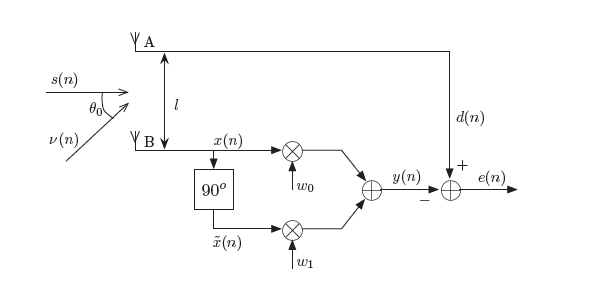
\includegraphics[width=0.5\textwidth]{antenna_array.png}
\caption{\label{fig:antenna_array}A two-element antenna array.}
\end{figure}

The beamformer coefficients, h0 and h1, are selected (adapted), so that the difference
$$e(n) = d(n) − h^Tx(n)$$
where $h = [h0 h1]^T$, is minimized in the mean-square sense. The error signal e(n) is the
beamformer output.
For a given set of the beamformer coefficients w0 and w1 and a signal arriving at an
angle $\theta$, the array power gain, $G(\theta)$, is defined as the ratio of the signal power in the
output e(n) to the signal power at one of the omnis. Assuming that a narrow-band signal
$\gamma (n) cos n\omega_o$ is arriving at an angle $\theta$,
\begin{align*}
e(n) &= \gamma (n)[cos(n\omega_o − \pi sin \theta) − h0 cos n\omega_o − h1 sin n\omega_o]\\
&= \gamma (n)[(cos(\pi sin \theta) − h_0) cos n\omega_o + (sin(\pi sin \theta) − h_1) sin n\omega_0]\\
&= a(\theta)\gamma (n) sin(n\omega_o+ \varphi(\theta))
\end{align*}

where
$$a(\theta) = (cos(\pi sin \theta) − h_0)2 + (sin(\pi sin \theta) − h_1)2$$
and
$$\varphi(\theta) = tan^{−1}(\frac{cos(\pi sin \theta) − h_0}{sin(\pi sin \theta) − h_1}) $$


Using these, we get
$$G(\theta) = a^2(\theta) = (cos(\pi sin \theta) − h_0)2 + (sin(\pi sin \theta) − h_1)2$$
$G(\theta)$ when plotted against the angle of arrival of the received signal is called directivity
pattern of the array (beamformer).



\section{LMS Algorithm: Steepest Descent Technique}
$E^{2}=E[ |e[n]|^2]$ is a quadratic function of filter weights. Hence it contains only one extrma. We find the minimum of the mean square using the steepest descent technique as follows
$$ h[i+1] = h[i] - \mu\nabla E^{2} \Big \rangle _{h=h[i]}$$
Where $\mu$ is step size and $\nabla$ is gradient. 
We know that $\nabla E^{2}=[2Rh-2p]\Big \rangle _{w=w[i]}$
$$  h[i+1] = h[i] + \mu[2Rh-2p]\Big \rangle _{h=h[i]}$$
Suppose we replace $R=E[x[n]x^T[n]]$ by a very crude estimate $R=x[n]x^T[n]$ and P by $x[n]d[n]$.
Even though our estimates are really crude we will prove that the algorithm works even with such estimates.
In the above equation we need to know R and P; and hence it can only be used for offline applications. To derive an algorithm that works in realtime, we do the following: 
The previous weights in the iterative procedure will be convolved with $x[n-1],x[n-2],...$ and will contain information about a large number of $x[i]'s$
Therefore the equation becomes 
$$  h[n+1] = h[n] + \mu[n]e[n] $$
This algorithm is called the LMS algorithm.
Suppose we have exact P and R, $h[n+1]$ will converge directly to $h_{opt}$.
But we have crude estimate of P and R and hence $h[n+1]$ doesnt converge exactly to $h_{opt}$.

Convergence in mean of LMS algorithm

Consider $\Delta[n]= W[n]W_opt$ weight error vector
$$  w[i+1] = w[i] + \mu ex[n]e[n] $$
Subtracting $W_{opt}$ from both sides,
$$  \nabla[n+1] = \nabla[n] + \mu x[n]e[n] $$
But $ e[n]=d[n]-y[n] = d[n]-x^T[n]W[n]$
$$  w[n+1] = w[n] + \mu ex[n][d[n]-x^T[n](W_{opt}+\nabla[n])]$$
Say $E[\nabla(n)]=U[n]$
Taking expectation on both sides :
$$  v[n+1] = v[n] + \mu [P -R_{opt}]-\mu E[x[n]x^T[n]\nabla[n]]$$
We know that $W_{opt}=R^{-1}P \Rightarrow RW_{opt}=P$
$$  v[n+1] = v[n] -\mu E[x[n]x^T[n]\nabla[n]]$$

We invoke independence assumptions - 
Assume $w[n]$ is statistically independent of $x[n] and d[n]$
\begin{align*}  v[n+1] &= v[n] -\mu E[x[n]x^H[n]]e[\nabla[n]] \\
  v[n+1] &= v[n] -\mu Rv[n] \\
  v[n+1] &= v[n] -\mu E[x[n]x^T[n]\nabla[n]] \end{align*}
R is Hermitian positive semi-definite.
$R=TDT^H$
\begin{align*}  v[n+1] &= v[n](TIT^{H} - \mu TDT^{H})
\\  v[n+1] &= T(I-\mu D)T^Hv[n]
\\  u[n+1] &= T(I-\mu D)u[n]\end{align*}
Normalization of a vector doesnt change when multiplied by a unitary matrix
If we can show $\lim_{n\to\infty}||u[n]||=0$ ; then $w[n]$ will converge to $W_{opt}$ in the mean.
$[I-\mu D]$ is a diagonal matrix
$$||u[n]||^2=\sum_{i=0}^{N}|1-\mu\lambda_i|^2|u_i[n]|^2 $$
We can choose $\mu$ such that $1-\mu\lambda_i < 1$
$$||u[n]||^2 < ||u[n+1]||^2$$
Normalization of $u[n]$ is monotonically decreasing 
But $||u[n]||^2\geq 0$
Hence $\lim_{n\to\infty}||u[n]||=0$
Choice of u is non-negative
$\lambda_i's$ are positive as R is Power spectral density.
We choose $\mu$ such that
\begin{align*} 0<(1-\lambda_i \mu)^2<1 
\\ -1<(1-\lambda_i\mu)<1
\\ 0<\mu<2/\lambda_{max}\end{align*}
We know that $R=TDT^H$
$$Trace(R)=Trace(D)$$
$$\sum \geq \lambda_max$$





\end{document}